\chapter{Hibridación de Métodos de Programación Matemática con Algoritmos Evolutivos} \label{Chapter6} 


En los Capítulos \ref{Chapter3} y \ref{Chapter4} se presentan dos esquemas importantes en cuanto al diseño de algoritmos en el área de la optimización, específicamente en la optimización de problemas con espacios de búsqueda continuos. En el primer esquema se tienen los algoritmos clásicos de programación matemática los cuales son eficientes buscadores locales, y  en el segundo se encuentran algoritmos evolutivos, los cuales utilizan una población de individuos (soluciones candidatas) que les permite obtener información global sobre el espacio de búsqueda. Teniendo en cuenta estos dos esquemas, este capítulo describe la propuesta de solución diseñada durante la presente investigación.

La calidad del desempeño de un algoritmo de optimización depende en gran medida del balance entre las operaciones de exploración y explotación del espacio de búsqueda que sean concebidas en su diseño. Cuando los operadores del algoritmo están orientados a la explotación, este puede quedar estancado en mínimos locales o bien ser sensible al punto de inicio debido a que sólo se conoce una región limitada del espacio de posibles soluciones. Sin embargo, los algoritmos con estas características presentan una mayor velocidad de convergencia al mínimo para espacios de búsqueda convexos. Por otra parte, un algoritmo con operadores mayormente exploratorios presentará generalmente una convergencia lenta y tiempos de ejecución altos; pero no será sensible al punto de inicio y la probabilidad de quedar estancado en mínimos locales será menor.

Debido a la diversidad de problemas en el área de la optimización este balance es difícil de lograr. Algunos problemas requerirán mayor explotación en regiones prometedoras para agilizar la búsqueda y en otros, se necesitará información global del espacio de búsqueda (operaciones de exploración) para encontrar la solución óptima. Esta cuestión es abordada en los teoremas de \textit{No Free Lunch} para la optimización, donde se plantea que si un algoritmo se desempeña particularmente bien en promedio para una clase de problemas, entonces debe hacerlo peor en promedio con respecto a los problemas restantes. En particular, si un algoritmo tiene mejor rendimiento que la búsqueda aleatoria en una clase de problemas, entonces debe tener un rendimiento peor que la búsqueda aleatoria en las clases de problemas restantes \cite{wolpert1997no}. En este sentido la hibridación puede resultar un enfoque efectivo para diseño de algoritmos más eficientes y que puedan resolver eficazmente un amplio espectro de problemas.

En el contexto de las metaheurísticas, la hibridación se refiere principalmente al proceso de combinar o integrar las mejores características de dos o más algoritmos, para formar uno nuevo que supere las partes originales en la resolución de un problema específico o un conjunto de problemas de referencia general \cite{Swagatam_2011}. Dragoi en \cite{Dragoi_2015} considera tres clasificaciones de hibridación de acuerdo a diferentes aspectos.
\begin{enumerate}
\item  Según los tipos de algoritmos que participan en la hibridación:
\begin{enumerate}
\item Metaheurísticas con metaheurísticas.
\item Metaheurísticas con algoritmos específicos del problema.
\item Metaheurísticas con métodos de programación matemática o inteligencia artificial (que, a su vez, pueden ser: técnicas exactas u otras heurísticas)
\end{enumerate}

\item Con respecto al nivel de hibridación, se encuentran dos casos:
\begin{enumerate}
\item Acoplamiento débil de alto nivel (los algoritmos conservan sus propias identidades)
\item Acoplamiento fuerte de bajo nivel (se intercambian componentes individuales)
\end{enumerate}

\item Cuando se toma en cuenta el orden de ejecución, la hibridación puede ser: 
\begin{enumerate}
\item  Secuencial.
\item  Intercalada.
\item  Paralela
\end{enumerate}
\end{enumerate}
De las siguientes clasificaciones se infiere la diversidad de investigaciones en el área de la hibridación. A continuación se presentan algunos trabajos de hibridación desde el enfoque que concibe una metaheurística como buscador global y un método directo de programación matemática como buscador local. Específicamente se destacarán los trabajos previos que se presentan los dos algoritmos utilizados en la propuesta de solución la Evolución Diferencial (buscador global) y el método de Nelder Mead como buscador local.
%%%%%%%%%%%%%%%%%%%%%%%%%%%%%%%%%%%%%%%%%%%%%%%%%%%%%%%%%%%%%%%%%%%%%%%%%%%%%%%%

\section{Hibridación de la Evolución Diferencial con Métodos de Búsqueda Local}

En el capítulo introductorio del presente trabajo se abordó el concepto de algoritmo memético (AM): un esquema que utiliza una metaheurística como algoritmo base de búsqueda global y que aplica métodos de búsqueda local para mejorar el rendimiento y refinar a los individuos en la población. Este tipo de hibridación es un enfoque integrador (coercitivo), ya que el algoritmo de búsqueda local se considera un subordinado y está incorporado en otro algoritmo \cite{raidl2006unified}. Diversos estudios muestran que, para algunos problemas, los AM son más eficientes y más efectivos que los AE tradicionales \cite{krasnogor2005tutorial}. Los trabajos de hibridación más destacados que combinan la ED y un método de programación matemática se encuentran dentro de este tipo de esquema y sirvieron como base para el enfoque propuesto.

En el artículo ``Algoritmo Integrado de Estrategias de Evolución Diferencial con Búsqueda Local''  (ISDE-L), se aplica un procedimiento de búsqueda local para mejorar el rendimiento \cite{elsayed2011integrated}. En en cada $k$ generaciones, se ordena la población según su valor de aptitud y se selecciona un individuo al azar del 25\% de la población. A este individuo se le aplica una técnica de búsqueda local con un número máximo de evaluaciones. La búsqueda local consiste en elegir aleatoriamente una variable del vector seleccionado, y luego se le suma o resta un número gaussiano aleatorio, como un tamaño de paso, tomándose la mejor dirección de acuerdo con la función de aptitud. Si el paso es exitoso y  mejora el individuo seleccionado, entonces el valor se actualiza. Este proceso continúa hasta que se seleccionan todas las variables o se alcanza el número máximo de evaluaciones. El algoritmo ISDE-L es aplicado al conjunto de problemas de prueba presentados en congreso CEC 2010. Los resultados obtenidos fueron mejores o iguales a los alcanzados por algoritmos de vanguardia para estos problemas prueba.

 Liao en \cite{liao2010two}, combina una versión de la ED modificada (MDE) con el método de Caminata Aleatoria con Dirección de Explotación (RWDE por sus siglas en inglés) como el operador de búsqueda local para mejorar los vectores $x_{r_1}$,$x_{r_2}$ y $x_{r_3}$ en la mutación diferencial. RWDE es un método iterativo de optimización estocástica que genera una secuencia de aproximaciones al óptimo al asumir un vector aleatorio como una dirección de búsqueda. El algoritmo híbrido resultante es llamado MDE-LS (del inglés Modified Differential Evolution-Local Search) y es considerado por el autor como un algoritmo memético. Se seleccionan un total de catorce problemas de diseño de ingeniería encontrados en literatura en diferentes campos de ingeniería. En siete de los catorce problemas, el algoritmo MDE-LS encuentra el óptimo global dentro del error 10E-6 en treinta ejecuciones. El algoritmo MDE-LS produce tasas de éxito más altas en 8 problemas pero menor en 2, en comparación con las del algoritmo MDE. En general, el MDE-LS mejora la tasa de éxito promedio en un 10\% sobre el algoritmo MDE.



En \cite{neri2008memetic}, se presenta una algoritmo memético que utiliza como buscador global la ED y dos algoritmos de búsqueda local, el Algoritmo Hooke-Jeeves (HJ) y el Buscador Local Estocástico (SLS por sus siglas en inglés). Los métodos de búsqueda local ayudan al marco evolutivo (ED) al ofrecer perspectivas exploratorias alternativas. El objetivo de ambos algoritmos es mejorar localmente una solución inicial explorando su vecindad. El espacio a explorar por los buscadores locales tiene un radio inicial. Luego, cuando no es posible  realizar una mejora, se genera una vecindad del espacio más pequeña reduciendo el radio. Para ambos algoritmos de búsqueda local, se establece un presupuesto igual a 300 evaluaciones de la función de aptitud. Los resultados estadísticos muestran que los MA presentados son competitivos con la ED y no requieren un ajuste de parámetros que podría terminar siendo costoso en términos de recursos de cómputo. 

Rogalsky y Derksen en \cite{rogalsky2000hybridization} proponen un algoritmo híbrido que combina el método el descenso simple (DS) con la ED para de acelerar la convergencia del algoritmo, sin que este quede atrapado en los mínimos locales.
DS es un método de búsqueda local basado en simplex que utiliza operadores de reflexión, expansión y contracción. La versión híbrida, denotada HDE utiliza los tres mecanismos.
De cada generación resultante de la aplicación de la ED, se eligen $ n + 1 $ individuos para formar un simplex. Esto puede realizarse de diferentes formas ya sea seleccionando los $n+1$ mejores, peores o aleatoriamente. A través de los operadores de DS, el simplex se modifica hasta que uno (o varios) individuos se mejoran. Todos los vectores mejorados se eligen para pasar a la siguiente generación. 

Wang en \cite{wang2011parameter}, combina la búsqueda realizada por DE con el método Nelder-Mead  en un algoritmo híbrido que es aplicado a la identificación de parámetros de varios sistemas caóticos. En cada generación se realizan cuatro pasos principales: primero los $P$ individuos de la población son ordenados de acuerdo su valor de aptitud. Luego, los primeros $Q$ individuos se usan para calcular el centroide del simplex. En el tercer paso, se realiza por cada uno de los restantes P-Q individuos, una iteración del NM con el centroide calculado mediante los Q mejores individuos. Aquí, la información de los mejores individuos es utilizada para guiar la búsqueda local del algoritmo. Por lo tanto, se modifica la búsqueda clásica de NM simplex, que se utiliza para guiar la búsqueda hacia regiones prometedoras. Luego se aplica la ED a toda la población $P$. Las simulaciones numéricas basadas en varios sistemas caóticos típicos y las comparaciones con otros enfoques existentes demostraron la efectividad, eficiencia y robustez del algoritmo híbrido propuesto. 



\section{Enfoque propuesto}\label{sec:Enfoque propuesto}
Como se puede observar en las investigaciones previas, la mayoría de los enfoques consisten en aplicar, bajo ciertas condiciones y con un número determinado de evaluaciones,  un método de búsqueda local a determinados individuos de la población para mejorar su valor de aptitud. La Evolución Diferencial siempre se aplica sobre toda la población y en la mayoría de las propuestas los métodos de búsqueda local no conocen información global en el momento de su aplicación. Sólo el caso de \cite{wang2011parameter} difiere en este sentido, ya que que el NM utiliza un centroide calculado con los mejores individuos. Sin embargo, esta propuesta realiza un número de evaluaciones por generación considerablemente mayor que la ED tradicional ya que se realizarán en cada generación $2(P-Q)$ evaluaciones de la función de aptitud debido a la aplicación de NM (el cual realiza dos evaluaciones en la versión sin operador de encogimiento) para luego realizar las $P$ evaluaciones de la ED. 

Teniendo en cuenta los trabajos de hibridación encontrados en la literatura especializada, la hipótesis y objetivos de la presente investigación, se diseña un nuevo enfoque de hibridación que pretende aumentar el equilibrio y la sinergia entre los buscadores global y local, así como la reducción del número de evaluaciones para disminuir la complejidad temporal. Los algoritmos híbridos presentados en próximas secciones fueron diseñados de acuerdo a los siguientes lineamientos de diseño:
\begin{enumerate}
\item Se distribuyen aleatoriamente $K$ instancias de un buscador local que cubrirán y explotarán el espacio de búsqueda.
\item Una instancia de un buscador global se utiliza para coordinar y compartir información entre las instancias del buscador local.
\item Las instancias del buscador local pueden incorporar información global o histórica en sus operadores.
\item El buscador local se aplica a un subconjunto del total de individuos de la población en cada generación.
\item El buscador global se aplica a cierto subconjunto del total de la población en cada generación.
\item La información de todos individuos en la población es utilizada en cada generación.
\item El trabajo debe ser balanceado: el número de evaluaciones destinadas a los buscadores local y global debe ser equilibrado para garantizar un balance entre la exploración y explotación.
\end{enumerate}
\newpage
La novedad del enfoque propuesto radica en la dinámica establecida entre ambos buscadores. A diferencia de los enfoques identificados en la literatura, este enfoque delega mayor participación al buscador local, aunque no existe subordinación de ningún algoritmo. Al distribuir diferentes instancias del buscador local se garantiza una mayor exploración del espacio de búsqueda en las primeras generaciones y una explotación exhaustiva de la región más prometedora en las generaciones finales.

El hecho de que los buscadores locales utilicen información global o histórica en sus operadores (mejor o peor individuo, individuos seleccionados aleatoriamente de la población, historial de mejores o peores individuos, etcétera), reduce la probabilidad de estancamiento o de convergencia prematura de las instancias. Por tanto, los buscadores locales deberán ser adecuadamente modificados para garantizar esta característica. 

Por otra parte, tanto las instancias de los buscadores locales como el buscador global no se aplicarán a todos los individuos de la población sino un subconjunto de la misma, lo que reduce el número de evaluaciones realizadas en cada generación. Tanto la característica anterior como la directriz del trabajo balanceado, implica que el buscador local a utilizar debe realizar un número relativamente pequeño de evaluaciones por iteración en comparación con el buscador global. De lo contrario, el número de instancias del buscador local deberá ser reducido, lo implicaría explotar menos regiones del espacio de búsqueda. 

En las siguientes secciones se describen las variantes híbridas que constituyen las propuestas de solución del presente trabajo de investigación. Estos algoritmos integran la Evolución Diferencial como buscador global y el método de Nelder-Mead buscador local bajo este enfoque de hibridación. El método NM fue modificado mediante el diseño experimental para lograr la hibridación. Nuevos operadores son agregados, los cuales conciben aleatoriedad e insertan información sobre regiones del espacio de búsqueda que se encuentran fuera de la vecindad en que trabaja la instancia el buscador local.

\subsection{Método de Nelder Mead con Expansión de Longitud Aleatoria: NMELA} \label{sec:NMELA}
Se selecciona el método Nelder Mead para llevar a cabo la hibridación por tres razones principales. La primera se debe a la capacidad del Nelder Mead para recolectar información de un área local del espacio de búsqueda realizando pocas evaluaciones de la función objetivo. El nuevo simplex en la i-ésima iteración contiene sólo un nuevo vértice: el punto aceptado que reemplaza al peor vértice en el simplex anterior. Este punto es generado a partir del punto reflejado por el peor, por lo tanto en cada iteración el método Nelder Mead realiza dos evaluaciones de la función objetivo. En el caso de las variantes planteadas a continuación, se realizan cuatro evaluaciones de la función objetivo como máximo por iteración. 

La segunda razón es la complejidad temporal del método NM original. Debido al hecho de que, el simplex en la  i-ésima iteración fue objeto de ordenamientos en iteraciones anteriores, la complejidad temporal del ordenamiento raras veces llega al peor caso. Por tanto, el orden de los vértices se puede realizar en tiempo lineal (a lo sumo $n$ comparaciones) en un paso de ordenación de inserción por ejemplo. El nuevo centroide también se calcula actualizando el anterior en una operación de sumatoria con complejidad de $O(n)$, con poco espacio  adicional de almacenamiento en memoria \cite{Singer2018}. 

La tercera razón se debe a los resultados experimentales obtenidos por las versiones aleatorizadas descritas en el Capítulo \ref{Chapter7}, Sección \ref{sec:Experimento A: Pruebas de estadísticas sobre el Método Nelder-Mead con Expansión de Longitud Aleatoria}. Al aumentar la capacidad de exploración mediante expansiones con longitud aleatoria ( las cuales pueden llegar a ser más largas que la expansión original), se evidencia un aumento significativo del desempeño con respecto al método original para todos los problemas de diseño cinemático.

Con el objetivo de explorar cuáles serían los beneficios de agregar cierta diversidad en los movimientos del simplex se realizaron tres versiones del Nelder Mead original (Véase Algoritmo \ref{alg:Nelder Mead}). Las versiones consisten en aplicar operadores basados en el operador de expansión original pero con longitudes aleatorias que permiten diversificar la búsqueda, expandiendo un simplex pequeño para lograr el escape de mínimos locales. Se realizaron modificaciones para el manejo de restricciones aplicando las reglas de Deb para comparar los puntos del simplex (Véase \cite{deb_efficient_1998}), y una regla de acotamiento para las variables de diseño. El simplex inicial fue generado de forma aleatoria, y se utilizaron los parámetros  $\gamma$ y $\beta$ de acuerdo a las características del problema. La condición de parada fue cambiada por el número de evaluaciones con la finalidad de medir el rendimiento. 

\subsubsection{Operador de Expansión con Longitud Aleatoria}

El primer operador propuesto se aplica cuando ninguno de los operadores del método original mejoran, de acuerdo a las reglas de Deb, al peor punto $x_h$ . Entonces, se realiza una expansión  donde el factor $\gamma$ es sustituido por dos números aleatorios para cada miembro del operador. Como coeficiente de   $x_c$, se emplea un número aleatorio determinado dado por la ecuación $C =1+c_1(N+1)$ donde $N$ es el número de variables y $c_1 \in (0,1)$ es un número aleatorio. Como coeficiente del punto $x_h$ se emplea un número aleatorio $c_2 \in (0,1)$. Se puede observar que el tamaño de la longitud de la expansión será proporcional a la dimensionalidad del problema. La Ecuación \ref{eq:NMELA} refleja el operador de Expansión de Longitud Aleatoria (ELA). El método NM modificado con el operador ELA se describe en el Algoritmo \ref{alg:NMELA}. Donde $NE$ es el número máximo de evaluaciones a realizar, $E$ es el contador de evaluaciones, la función $es\_mejor(x_1,x_2)$  retorna verdadero si el primer argumento es mejor que el segundo de acuerdo a las reglas de Deb.
\begin{center}
\begin{equation}\label{eq:NMELA}
x_{new}=(1+c_1(N+1))x_c-c_2 x_h
\end{equation}
\end{center}

\begin{algorithm}\label{alg:NMELA}
	\begin{algorithmic}
		\STATE Elegir parámetros: $\beta>0, \gamma \in (0,1)$
		\STATE Generar un simplex inicial de forma aleatoria.
        \STATE Evaluar simplex inicial
        \STATE Hacer $E=N+1$.
		\label{lin:lineaRara}
		\WHILE {$E<NE$}
		\STATE Ordenar los puntos del simplex según $es\_mejor(x_1,x_2)$ .
		\STATE Elegir $x_h$ (peor punto), $x_l$ (mejor punto) y $x_g$ (el segundo peor punto).
		
		\STATE Calcular $x_c=\frac{1}{N} \sum_{i=1, i\neq h }^{N+1} x_i$
		\STATE Realizar la reflexión $x_r=2x_c -x_h$
        \STATE Acotar  $x_r$
        \STATE Evaluar  $f(x_r)$
        \STATE Hacer  $E=E+1$

		\IF{$es\_mejor(x_r,x_l)$}
		\STATE Hacer $x_{new}=(1+\gamma)x_c-\gamma x_h$ (Expansión)
		\ELSE \IF {$es\_mejor(x_h,x_r)$}
		\STATE Hacer $x_{new}=(1-\beta)x_c+\beta x_h$ (Contracción adentro)
		\ENDIF
		\ELSE \IF {$es\_mejor(x_r,x_g) \quad \AND \quad es\_mejor(x_h,x_r)$}
		\STATE Hacer $x_{new}=(1+\beta)x_c-\beta x_h$ (Contracción afuera)
		\ENDIF
		\ENDIF
        \STATE Acotar  $x_{new}$
        \STATE Evaluar  $f(x_{new})$
        \STATE Hacer $E=E+1$
		\IF {$es\_mejor(x_h,x_{new})$}
		\STATE Calcular  $x_{new}=(1+c_1(N+1))x_c-c_2 (x_h)$ (ELA)
        \STATE Acotar  $x_{new}$
        \STATE Evaluar  $f(x_{new})$
        \STATE Hacer $E=E+1$

		\ENDIF
		\ENDWHILE
	\end{algorithmic}
	\caption{Método de Nelder-Mead con Expansión de Longitud Aleatoria}\label{alg:NMELA}
\end{algorithm}

\subsubsection{Operador de Expansión Inversa con Longitud Aleatoria }\label{NMEILA}
El segundo operador propuesto se aplica de forma similar al operador ELA. Cuando ninguno de los operadores del algoritmo original mejoran el peor punto se realiza una expansión con longitud aleatoria, sólo que en este caso se toma al mejor punto $x_l$ para expandir en lugar de $x_h$.

El objetivo de realizar esta operación es hacer un movimiento drástico para escapar del estancamiento probando direcciones contrarias al mejor que se asume como mínimo local. En caso de que el punto encontrado no mejore al peor punto, será utilizado como peor en las iteraciones siguientes y mejorado con los operadores clásicos del método, ya sea por reflexión o expansión. En cualquier caso, el operador permite probar nuevas direcciones en el espacio de búsqueda y aumentar la diversidad del simplex, una vez que este se encuentra ``cerrado'' sobre un mínimo local. En la Ecuación \ref{eq:NMEILA} se describe el operador de Expansión Inversa de Longitud Aleatoria (EILA). El Algoritmo \ref{alg:NMEILA} describe la modificación del Nelder Mead original con el operador en cuestión.
\begin{center}
\begin{equation}\label{eq:NMEILA}
x_{new}=(1+c_1(N+1))x_c-c_2x_l
\end{equation}
\end{center}

\begin{algorithm}
	\begin{algorithmic}[1]
		\STATE Elegir parámetros: $\beta>0, \gamma \in (0,1)$
		\STATE Generar un simplex inicial de forma aleatoria.
		\STATE Evaluar simplex inicial
        \STATE Hacer $E=N+1$.
		\WHILE {$I<NE$}
		\STATE Ordenar los puntos del simplex.
		\STATE Elegir $x_h$ (peor punto), $x_l$ (mejor punto) y $x_g$ (el segundo peor punto).
		\STATE Calcular $x_c=\frac{1}{N} \sum_{i=1, i\neq h }^{N+1} x_i$
		\STATE Realizar la reflexión $x_r=2x_c -x_h$
		\IF{$es\_mejor(x_r,x_l)$}
		\STATE Hacer $x_{new}=(1+\gamma)x_c-\gamma x_h$ (Expansión)
		\ELSE \IF {$es\_mejor(x_h,x_r)$}
		\STATE Hacer $x_{new}=(1-\beta)x_c+\beta x_h$ (Contracción adentro)
		\ENDIF
		\ELSE \IF {$es\_mejor(x_r,x_g) \quad \AND \quad es\_mejor(x_h,x_r)$}
		\STATE Hacer $x_{new}=(1+\beta)x_c-\beta x_h$ (Contracción afuera)
		\ENDIF
		\ENDIF
        \STATE Acotar  $x_{new}$
        \STATE Evaluar  $f(x_{new})$
        \STATE Hacer  $E=E+1$
		\IF {$es\_mejor(x_h,x_{new})$}
		\STATE Calcular  $x_{new}=(1+c_1(N+1))x_c-c_2 (x_l)$ (EILA)
        \STATE Acotar  $x_{new}$
        \STATE Evaluar  $f(x_{new})$
        \STATE Hacer  $E=E+1$
		\ENDIF
		\ENDWHILE
	\end{algorithmic}
	\caption{Método de Nelder-Mead con Expansión Inversa de Longitud Aleatoria}\label{alg:NMEILA}
\end{algorithm}

\subsubsection{Combinación de los operadores}
Una versión final del NM se realizó combinando los dos operadores. Al igual que en las versiones anteriores, si los operadores originales no logran mejorar el peor punto, primero se realiza el operador descrito en la Ecuación \ref{eq:NMELA} , y si este no supera al peor punto se aplica el operador que refleja el mejor punto descrito en el Ecuación \ref{eq:NMEILA}. Esta combinación de operadores se realiza con el propósito de probar más direcciones de búsqueda y alcanzar mayor capacidad de exploración en el método NM. El Algoritmo \ref{alg:NM2ELA} describe la versión del método NM con dos Operadores de Expansión con Longitud Aleatoria (NM2ELA). 

\begin{algorithm}
	\begin{algorithmic}[1]
		\STATE Elegir parámetros: $\beta>0, \gamma \in (0,1)$. 
		\STATE Generar un simplex inicial de forma aleatoria.
        \STATE Evaluar el simplex inicial
        \STATE Hacer $E=N+1$
		\label{lin:lineaRara}
		\WHILE {$E<NE$}
		\STATE Ordenar los puntos de acuerdo a las reglas de Deb.
		\STATE Elegir $x_h$ (peor punto), $x_l$ (mejor punto) y $x_g$ (el segundo peor punto).
		\STATE Calcular $x_c=\frac{1}{N} \sum_{i=1, i\neq h }^{N+1} x_i$
		\STATE Realizar la reflexión $x_r=2x_c -x_h$
		\IF{$es\_mejor(x_r,x_l)$}
		\STATE Hacer $x_{new}=(1+\gamma)x_c-\gamma x_h$ (Expansión)
		\ELSE \IF {$es\_mejor(x_h,x_r)$}
		\STATE Hacer $x_{new}=(1-\beta)x_c+\beta x_h$ (Contracción adentro)
		\ENDIF
		\ELSE \IF {$es\_mejor(x_r,x_g) \quad \AND \quad es\_mejor(x_h,x_r)$}
		\STATE Hacer $x_{new}=(1+\beta)x_c-\beta x_h$ (Contracción afuera)
		\ENDIF
		\ENDIF
		\IF {$es\_mejor(x_h,x_{new})$}
		\STATE Calcular  $x_{new}=(1+c_1(N+1))x_c-c_2 (x_h)$ (ELA)
		\ENDIF
        \STATE Acotar   $x_{new}$
        \STATE Evaluar  $f(x_{new})$
        \STATE Evaluar  $E=E+1$
        \IF {$es\_mejor(x_h,x_{new})$}
		\STATE Calcular  $x_{new}=(1+c_1(N+1))x_c-c_2 (x_l)$ (EILA)
        \STATE Acotar   $x_{new}$
        \STATE Evaluar  $f(x_{new})$
        \STATE Evaluar  $E=E+1$
		\ENDIF
		\ENDWHILE
	\end{algorithmic}
	\caption{Método de Nelder-Mead con dos operadores de Expansión con Longitud Aleatoria}
    \label{alg:NM2ELA}
\end{algorithm}

\subsection{Observaciones Preliminares}

Los resultados obtenidos durante el diseño experimental (Véase Sección \ref{sec:Experimento A: Pruebas de estadísticas sobre el Método Nelder-Mead con Expansión de Longitud Aleatoria} ) muestran tanto potencialidades como desventajas del NM. Aumentando la probabilidad de expansiones más largas tanto por la reflexión del peor punto como por la reflexión del mejor, se logra aumentar la eficiencia del método superando para MCE2, los resultados obtenidos por la ED (2.6280E-03) en el mejor punto con \textbf{3.8126E-04} para NM2ELA. Es importante destacar que el nuevo mínimo esta dado por un vector distante al encontrado por la ED y representa un mecanismo completamente diferente, lo que indica un aumento en la capacidad de exploración del método. 

Otra de las bondades de estos operadores es que aumentan la robustez ( sobre todo para baja dimensionalidad), con respecto al NM clásico, que queda demostrado en las medidas de tendencia central y de dispersión, siempre superiores al método original. El número de evaluaciones es significativamente menor al utilizado por la ED pues debido a la rápida convergencia del NM no se encontraron diferencias de desempeño al realizar mayor cantidad de evaluaciones. 

Además, las pruebas de Friedman y Bonferroni (Véase Figura \ref{fig: Bonferroni-Dunn -NMELA}), establecen que  las variantes propuestas presentan un desempeño significativamente superior con respecto a dos versiones deterministas del NM, para los cinco primeros problemas de optimización correspondientes al diseño cinemático.

De forma general, se observa que la dimensionalidad del espacio vectorial impacta significativamente en el desempeño del método, característica que ya ha sido reportada en trabajos previos y que se confirma en el presente \cite{han_effect_2006}. Para los problemas con $N>10$ el algoritmo muestra un comportamiento más errático en los resultados de sus ejecuciones, las cuales comienzan a diferir unas de otras. 

 Las variantes aleatorizadas pueden encontrar valores cercanos, iguales o mejores a los mínimos ya reportados, a diferencia  de las versiones deterministas. Sin embargo, las medidas de tendencia central son distantes a las obtenidas por las variantes de la ED, sobre todo para los problemas de mayor dimensión. Por tanto, se evidencia que a pesar de las mejoras en el rendimiento, las versiones aleatorizadas aún son sensibles al punto de inicio (simplex inicial) y continúan siendo métodos de búsqueda local. Esta deficiencia puede ser atacada mediante un enfoque poblacional, de acuerdo a los lineamientos propuestos en la Sección \ref{sec:Enfoque propuesto} para lograr un mayor cubrimiento del espacio de búsqueda en las iteraciones tempranas.

%%%%%%%%%%%%%%%%%%%%%%%%%%%%%%%%%%%%%%%%%%%%%%%%%%%%%%%%%%%%%%%%%%%%%%%%%%%%%%%%%%%%%%%%%%%%%%%%%%%%%%%%%%%

\subsection{Algoritmo Híbrido basado en el Método Nelder Mead con Evolución Diferencial: HNMED. Variante I}\label{sec:HNMEDV1}
Las etapas iniciales del diseño experimental resultaron en el diseño e implementación del Algoritmo Híbrido basado en el Método Nelder  Mead con Evolución Diferencial: HNMED. El procedimiento general  consiste en dividir una población $X$ generada de forma aleatoria en exactamente $NS$ símpleces o sub-poblaciones de tamaño $N+1$. En la generación $G$, cada instancia $k=\{1,2,...,NS\}$ del NM realizará una búsqueda local utilizando el simplex $S_k$. Luego, se aplica la ED utilizando como individuo padre el mejor punto $x^k_l$ del simplex $S_k$. Los individuos seleccionados aleatoriamente para realizar la mutación diferencial ($x_{r_1}$,$x_{r_2}$,$x_{r_1}$), se eligen de toda la población $X$. Se selecciona como buscador global la ED/rand/1/bin debido a que el operador sólo utiliza información global para realizar la mutación diferencial. En la primera variante se utiliza como buscador local la versión aleatorizada del NM con el operador NMEILA descrito en la Sección \ref{NMEILA}.

El diseño se basa en el enfoque de hibridación planteado al inicio del presente capítulo. Al dividir la población en varios símpleces, se garantiza una explotación de diferentes regiones del espacio de búsqueda mediante varias instancias del buscador local. El método NM resulta una opción adecuada ya que al utilizar el simplex para realizar sus operaciones, es capaz recolectar información de un área limitada del espacio del búsqueda mediante el cálculo del centroide. Por tanto, para cada ejecución de una instancia del NM se utiliza información de todo el subconjunto de individuos a su disposición pero sólo se opera sobre el peor y se realizan tres evaluaciones de la función objetivo. Esto implica que en cada generación se realizarán $3NS$ evaluaciones en total, por parte de los buscadores locales.

La ED también opera siguiendo las reglas del enfoque propuesto. En cada generación, la ED se aplica a una sub-población de tamaño $NS$ integrada por los mejores individuos de cada simplex: $X_l=\{x^1_l,x^2_l,...,x^{NS}_l \}$. Sin embargo, para realizar la mutación diferencial se utiliza información de la población, seleccionando aleatoriamente los tres individuos para generar el vector ruido  de toda la población. De esta forma, la ED realiza $NS$ evaluaciones de la función objetivo por cada generación. 

En resumen, en una generación de HNMED se realizan un total $3NS+NS=4NS$ evaluaciones entre las $NS$ instancias del NM y la ED/rand/1/bin. La proporción entre las evaluaciones realizadas por el buscador local y global se encuentra dada por la relación $\frac{E_{ED}}{E_{NM}}=\frac{1}{4}$. El buscador local tiene mayor carga ya que constituye el método base que garantizará mayor rapidez. Sin embargo, su presupuesto de evaluaciones por generación no es excesivamente superior, de modo que se cumple el lineamiento del trabajo balanceado. 

Teniendo en cuenta que el tamaño de la población es $NP=(N+1)NS$, y que un algoritmo ED convencional realiza $NP$ evaluaciones por generación, la proporción entre las cantidad evaluaciones es:
\begin{equation}\label{eq:relación de evaluaciones}
\frac{E_{HNMED}}{E_{ED}}=\frac{4NS}{(N+1)NS}=\frac{4}{N+1}
\end{equation}
Nótese que, a medida que aumenta la dimesionalidad, el número de evaluaciones en cada generación realizadas por HNMED representarán un porcentaje cada vez menor con respecto a las realizadas por la ED. Por ejemplo, para el problema MCE2 ($N=6$) las evaluaciones por iteración de HNMED representan el 57\% ($\frac{4}{6+1}=0.57$) de las realizadas por la ED; para los casos GCE1 y GCE2 con $N=14$, el 26.7 \%($\frac{4}{14+1}=0.267$); para el problema MCE1 el 25\% ($\frac{4}{15+1}=0.25$), el 20\% ($\frac{4}{19+1}=0.20$) para MCE3 y así sucesivamente.

La Figura \ref{fig:HNMED} describe el esquema general de las variantes híbridas propuestas. Se pueden observar los diferentes símpleces que cubren diferentes áreas del espacio de búsqueda. Los mejores puntos de cada simplex son mejorados por la ED con información global acercándolos a regiones prometedoras en las primeras generaciones y reuniéndolos sobre el mínimo global en las iteraciones finales.

	\begin{figure}[htb]
		\begin{center}
		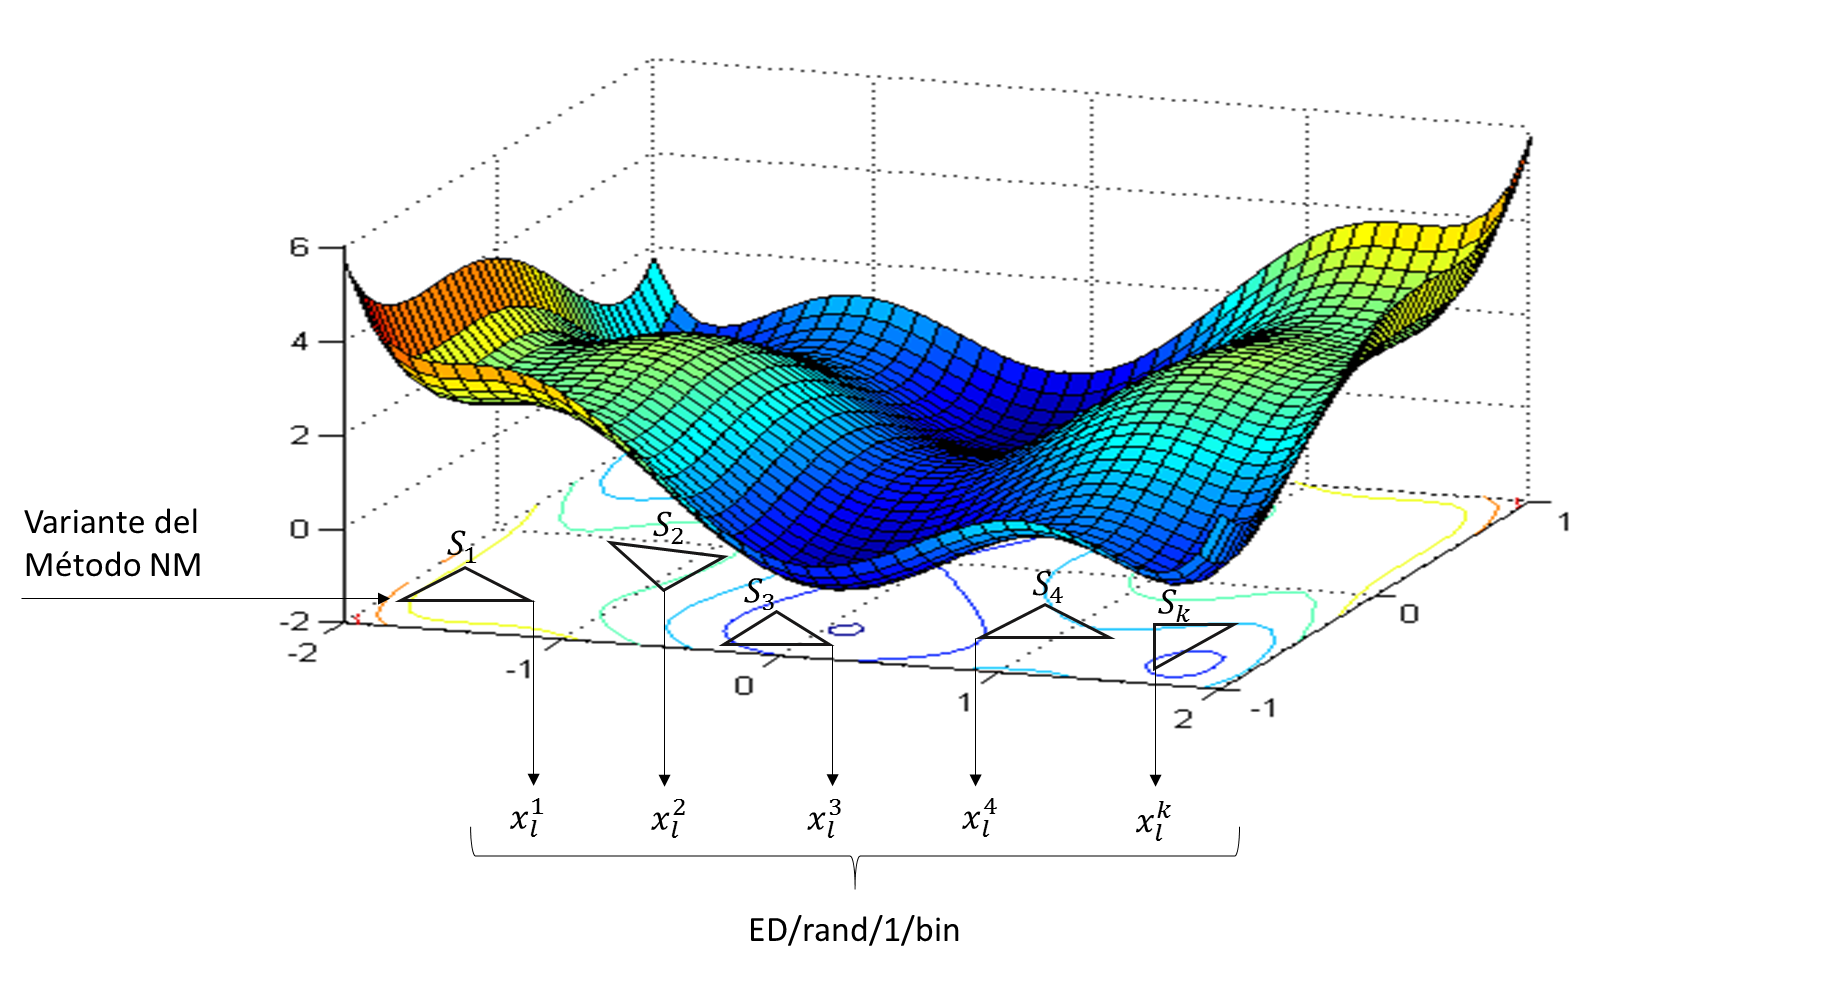
\includegraphics[width=\textwidth]{Figures/Esquema}
		\caption{Esquema de las variantes HNMED.}
		\label{fig:HNMED}
	\end{center}
	\end{figure}


El Algoritmo \ref{alg:HNMED} describe el pseudocódigo para las variantes HNMED. Las flechas rojas en las lineas desde la 26 a la 28 indican el fragmento de código que varía en cada una de las versiones. Donde $NE$ es el número máximo de evaluaciones, $NP$ es el tamaño de la población e $I_{x_l^k}$ el índice correspondiente al punto $x_l^k$ de $S_k$ en la población $X$. En las siguientes secciones se presentan cuatro variantes híbridas bajo el mismo enfoque, las cuales sólo difieren en el operador con aleatoriedad que incluye el método NM. Por tanto, solo se describirán dichos operadores; para mayor detalle sobre la implementación de estas variantes consultar el Anexo \ref{AppendixA}. 


\begin{algorithm}
	\begin{algorithmic}[1]
		\STATE Elegir parámetros: $\beta>0, \gamma \in (0,1)$
		\STATE Generar y evaluar una población aleatoria $X$ inicial.
        \STATE Hacer $E=NP$.
		\WHILE {$E<NE$}
           \STATE Generar $F=(0.3,0.9)$ y $CR=(0,0.8)$
           \FOR{$k \in \{1,\dots,NS\}$}
              \STATE Seleccionar $S_k$ de $X$
              \STATE Ordenar los puntos en $S_k$ de acuerdo a las reglas de Deb.
              \STATE Elegir $x^k_h$, $x^k_l$ y $x^k_g$.
              \STATE Calcular $x^k_c=\frac{1}{N} \sum_{i=1, i\neq h }^{N+1} x^k_i$
              \STATE Realizar la reflexión $x^k_r=2x^k_c -x^k_h$
              \STATE Acotar  $x^k_r$ y evaluar  $f(x^k_r)$
              \IF{$es\_mejor(x^k_r,x^k_l)$}
              \STATE Hacer $x_{new}=(1+\gamma)x^k_c-\gamma x^k_h$ (Expansión)
              \ELSE \IF {$es\_mejor(x^k_h,x^k_r)$}
              \STATE Hacer $x^k_{new}=(1-\beta)x^k_c+\beta x^k_h$ (Contracción adentro)
              \ENDIF
              \ELSE \IF {$es\_mejor(x^k_r,x^k_g) \quad \AND \quad es\_mejor(x^k_h,x^k_r)$}
              \STATE Hacer $x_{new}=(1+\beta)x^k_c-\beta x^k_h$ (Contracción afuera)
              \ENDIF
              \ENDIF
              \STATE Acotar $x^k_{new}$ y evaluar $f(x^k_{new})$
            
              \IF {$es\_mejor(x_h,x_{new})$}

              \STATE $\color{red} \Rightarrow $  Calcular $x^k_{new}$ según la variante  
              \STATE $\color{red} \Rightarrow $ Acotar  $x^k_{new}$ y evaluar  $f(x^k_{new})$  
              \STATE $\color{red} \Rightarrow $ Hacer  $E=E+1$ 
              \ENDIF
              \STATE Seleccionar aleatoriamente índices $r_1 \neq r_2 \neq r_3 \neq I_{x^k_l} $
              \STATE Generar aleatoriamente el índice $randb(j)=(1,N)$ 
              \FOR{$j \in \{1,\dots,N\}$}
                \IF{($randb(j) \leq CR) \quad \OR \quad (j==randb(j))$}
              	   \STATE $u^k_{j} = x_{r_1} + F (x_{r_2}-x_{r_3})$
              	\ELSE 
                  \STATE $u^k_{j} = x^k_{l_j}$
                \ENDIF
              \ENDFOR
             \STATE Acotar $u^k$ y evaluar $f(u^k)$
               \IF{ es\_mejor($f(u^k),x^k_l)$}
                  \STATE $x^k_l = u^k$
               \ENDIF
                 \STATE Hacer  $E=E+3$
        \ENDFOR
		\ENDWHILE
	\end{algorithmic}
	\caption{Algoritmo HNMED}\label{alg:HNMED}
\end{algorithm}

\subsubsection{HNMED. Variantes II y III}
La segunda variante difiere en la versión del NM utilizada. Si los operadores del Nelder Mead no mejoran al peor vector este se sustituye por un vector que tiene como base el mejor vector local $x^k_l$ y va hacia la dirección del mejor individuo en la población $best$ según describe la Ecuación \ref{eq:HNMED2-1}.
\begin{center}
\begin{equation}\label{eq:HNMED2-1}
x_{new}= x^k_l+ F(best-x^k_h)
\end{equation}
\end{center}
Este operador está basado en el cálculo del vector ruido de la mutación diferencial, nótese que $F$ es el mismo factor de escala utilizado en la mutación de la ED. En este caso, las instancias del Nelder-Mead tienen un operador que utiliza información global: el mejor individuo en la población. El objetivo aquí es acercar el peor punto en el simplex $S_k$ al mejor punto a nivel global de forma paulatina.

La tercera variante procede de la siguiente forma: dependiendo de cuál sea la mejor dirección, el vector ruido se dirigirá hacia el mejor punto a nivel global (Ecuación \ref{eq:HNMED2-1}) o se alejará del peor a nivel local con un tamaño de paso proporcional a la diferencia absoluta entre $best$ y $x^k_h$. Esta versión contiene el operador de la Variante II y agrega  un segundo operador (Ecuación \ref{eq:HNMED3-1}) que calcula un vector que tiene como base al mejor individuo local $x^k_l$ y que va en sentido contrario al peor vector local $x^k_h$.
\begin{center}
\begin{equation}\label{eq:HNMED3-1}
x_{new}= x^k_l- F(x^k_h-best)
\end{equation}
\end{center}
De forma similar a la estrategia seguida en NM2ELA el objetivo de utilizar dos operadores que presentan direcciones opuestas es aumentar la capacidad de exploración del buscador local y aumentar la diversidad en simplex para evitar convergencia prematura o estancamiento de las diferentes instancias.
\subsubsection{HNMED. Variantes IV y V }
Las últimas dos variantes están basadas en los operadores utilizados por la versión DE/current-to-best/1 para calcular el vector ruido. El propósito de estas variantes es evitar las dos evaluaciones de la variante III, incorporando más información global en el operador. Los vectores $x_{r_1}$,$x_{r_2}$ y $x_{r_3}$ son seleccionado aleatoriamente de toda la población y cumplen la condición de $ I_{x^k_l} \neq r_1 \neq r_2 \neq r_3$. Nótese que en el tercer miembro de la Ecuación \ref{eq:HNMED4-1} el factor de escala es $1-F$ el cual es el complemento de la probabilidad de $F$. Esta modificación se aplica con el objetivo de mantener un balance entre el miembro elitista y el aleatorio en el operador.
\begin{center}
\begin{equation}\label{eq:HNMED4-1}
%xl(1:n)+F*(best(1:n)-r1(1:n))+(1-F)*(r2(1:n)-r3(1:n))
x_{new}= x^k_l+F(best-x_{r_1})+(1-F)(x_{r_2}-x_{r_3})
\end{equation}
\end{center}
Los operadores propuestos hasta el momento utilizan como vector base un punto local ($x^k_l$). En la quinta variante, el operador utiliza como vector base uno de los vectores elegidos aleatoriamente, una vez más en la búsqueda de aumentar la exploración del espacio de búsqueda y mantener la diversidad de la población. El operador utilizado en la variante V se describe en la ecuación \ref{eq:HNMED5-1}
\begin{center}
\begin{equation}\label{eq:HNMED5-1}
%xl(1:n)+F*(best(1:n)-r1(1:n))+(1-F)*(r2(1:n)-r3(1:n))
x_{new}= x_{r_1}+F(best-x_{r_1})+(1-F)(x_{r_2}-x_{r_3})
\end{equation}
\end{center}
 %xnew1=r1(1:n)+F*(best(1:n)-r1(1:n))+(1-F)*(r2(1:n)-r3(1:n));
Diferentes variantes y combinaciones de estos operadores fueron implementadas. No obstante, se presentan las propuestas que mostraron un mejor rendimiento promedio para los problemas a resolver en la presente investigación. 
\\
\subsubsection{HNMED. Variante VI}
En el diseño inicial de las variantes HNMED se concibió la inicialización de la población de forma aleatoria de acuerdo al procedimiento del enfoque evolutivo. Sin embargo, se pasa por alto la naturaleza geométrica de los operadores utilizados por el Nelder-Mead. En \cite{spendley_sequential_1962}, Spendley plantea que un simplex inicial regular puede aumentar el desempeño de un método basado en simplex y plantea las fórmulas para generar un simplex regular de longitud $d$ tomando como centro del simplex un punto $c$ determinado. Por otra parte, Han y Neumann en \cite{han_effect_2006} comprueban que la tasa de convergencia $\rho$ del NM tiende a 1 a medida que aumenta respecto al número de variables $n$, esto es $ \lim_{n\to\infty}\rho(S_0,n)=1$. Incluso, los resultados experimentales muestran que para $\rho(S_0,32)=0.9912$, lo que indica que este efecto sucede rápidamente. Además, algunas consideraciones sobre el comportamiento del método NM original son presentadas: las operaciones de expansión y contracción producen una mayor reducción de la función que las operaciones de reflexión, y un simplex inicial de bordes más largos contribuye a una mejor minimización de la función objetivo. 

Teniendo en cuenta lo planteado en los párrafos anteriores y los resultados obtenidos durante la experimentación con las primeras variantes, se diseña un última versión (Véase Algoritmo \ref{alg:HNMEDV6}) que tiene como objetivo alcanzar una mayor capacidad de exploración en problemas de mayor dimensión. Dos modificaciones principales son llevadas a cabo respecto a las versiones anteriores:
\begin{enumerate}
	\item Se reemplaza la inicialización aleatoria de la población por el siguiente procedimiento: cada punto $x_i$ con $i =\left\lbrace  1,2,...,N+1\right\rbrace $ en  el simplex $S_k$ se genera de acuerdo a la siguiente formula:
	\begin{equation}\label{eq:Inicializacion de Simpleces}
	x^i_j=\begin{cases}
	\frac{u_j-l_j}{2}+p_j(\frac{u_j-l_j}{2}), & \text{si $i==j$}.\\
	u_j+q_k(\frac{u_j-l_j}{2})+r_j, & \text{en caso contrario}.
	\end{cases}
	\end{equation}
	Donde $u_j$ y $l_j$ son los limites superior e inferior en la dimensión $j$. Los valores de  $p_j$, $q_k$ y $r_j$ son números aleatorios de una distribución uniforme en los intervalos siguientes:
	\begin{equation}
	p_j \in \begin{cases}
	(0.05;5n/100), & \text{si $5n/100 <0.95$}.\\
	(0.05;0.95), & \text{en caso contrario}.
	\end{cases}
	\end{equation}
	
	\begin{equation}
	q_k \in \begin{cases}
	(0.5;3n/100), & \text{si $3n/100 <0.95$}.\\
	(0.05;0.95), & \text{en caso contrario}.
	\end{cases}
	\end{equation}
	\begin{equation}
	r_j \in (-NP/100,+NP/100) 
	\end{equation}
	La Ecuación \ref{eq:Inicializacion de Simpleces} esta basada en la presentada por Spendley en \cite{spendley_sequential_1962} para la generación de un simplex regular de longitud $d$, la cual fue concebida para un algoritmo que utiliza un solo simplex y no contempla la diversidad en las dimensiones requerida por la parte evolutiva para un desempeño correcto. Aquí se garantiza una distancia mínima entre los vértices del simplex los cuales se ubicarán en vecindades cercanas a los límites del espacio de búsqueda. Por ejemplo, el punto $x_1$ del simplex $S_k$  estará desplazado en su primera componente hacia región de longitud $(\frac{5n}{100}-0.05)\frac{u_1-l_1}{2}$ en la vecindad del límite superior de la primera dimensión. El punto $x_2$ desplazado hacia el límite superior de la segunda dimensión y así sucesivamente. Finalmente, el punto $x_{n+1}$ se ubicará en la vecindad $(\frac{3n}{100}-0.05)\frac{u_j-l_j}{2}$ de los límites inferiores en todas las dimensiones. El valor aleatorio $r_j$ se utiliza para garantizar una variación de los valores en la dimensión $j$ para el simplex $S_k$. El objetivo de esta inicialización de los símpleces es garantizar tetraedros más regulares y de mayor tamaño. 
	
	\item Las versiones iniciales de HNMED tenían un enfoque elitista. En el caso de HNMED-V4 y HNMED-V5 se utiliza la dirección del mejor para mejorar el peor punto de simplex y la ED sólo se aplicaba al los mejores puntos de cada simplex. Para garantizar que mayor cantidad de individuos reciban información global, los operadores son aplicados a una posición del simplex en cada generación ascendentemente. Esto es, que para la generación 1 la ED se aplica al individuo en la posición 1 en cada simplex, en la segunda generación al individuo en la posición 2 y así sucesivamente hasta llegar a la posición $NS+1$ donde se comienza de nuevo por la primera posición.  
	\item El operador de mutación diferencial utilizado es basado en DE/current-to-best/1:
	\begin{equation}
	v_m= x_m+F(x^r_l-x_{r_1})+(1-F)(x_{r_2}-x_{r_3})
	\end{equation}
	Donde el individuo elitista $x^r_l$ es seleccionado aleatoriamente del conjunto de los mejores individuos de cada simplex $X_l$. 
\end{enumerate}


\begin{algorithm}
	\begin{algorithmic}[1]
		\STATE Elegir parámetros: $\beta>0, \gamma \in (0,1)$
		\STATE $\color{red} \Rightarrow $ Generar símpleces según Ecuación \ref{eq:Inicializacion de Simpleces} y evaluar $X$.
		\STATE Hacer $E=NP$.
		\WHILE {$E<NE$}
		\STATE Generar $F=(0.3,0.9)$ y $CR=(0,0.8)$
		\FOR{$k \in \{1,\dots,NS\}$}
		\STATE Seleccionar $S_k$ de $X$
		\STATE Ordenar los puntos en $S_k$ de acuerdo a las reglas de Deb.
		\STATE Elegir $x^k_h$, $x^k_l$ y $x^k_g$.
		\STATE Calcular $x^k_c=\frac{1}{N} \sum_{i=1, i\neq h }^{N+1} x^k_i$
		\STATE Realizar la reflexión $x^k_r=2x^k_c -x^k_h$
		\STATE Acotar  $x^k_r$ y evaluar  $f(x^k_r)$
		\IF{$es\_mejor(x^k_r,x^k_l)$}
		\STATE Hacer $x_{new}=(1+\gamma)x^k_c-\gamma x^k_h$ (Expansión)
		\ELSE \IF {$es\_mejor(x^k_h,x^k_r)$}
		\STATE Hacer $x^k_{new}=(1-\beta)x^k_c+\beta x^k_h$ (Contracción adentro)
		\ENDIF
		\ELSE \IF {$es\_mejor(x^k_r,x^k_g) \quad \AND \quad es\_mejor(x^k_h,x^k_r)$}
		\STATE Hacer $x_{new}=(1+\beta)x^k_c-\beta x^k_h$ (Contracción afuera)
		\ENDIF
		\ENDIF
		\STATE Acotar $x^k_{new}$ y evaluar $f(x^k_{new})$
		
		\IF {$es\_mejor(x_h,x_{new})$}
		
		\STATE $\color{red} \Rightarrow $  Calcular  $x_{new}= x_{r_1}+F(best-x_{r_1})+(1-F)(x_{r_2}-x_{r_3})$
		\STATE Acotar  $x^k_{new}$ y evaluar  $f(x^k_{new})$  
		\STATE Hacer  $E=E+1$ 
		\ENDIF
		\STATE $\color{red} \Rightarrow $ Seleccionar aleatoriamente índices $r=$(1,N+1) y $r_1 \neq r_2 \neq r_3 \neq I_{x^k_l} $
		\STATE Generar aleatoriamente el índice $randb(j)=(1,N)$ 
		\FOR{$j \in \{1,\dots,N\}$}
		\IF{($randb(j) \leq CR) \quad \OR \quad (j==randb(j))$}
		\STATE $\color{red} \Rightarrow $ $u^k_{j} =  x^k_{mj}+F(x^r_l-x_{r_1})+(1-F)(x_{r_2}-x_{r_3})$
		\ELSE 
		\STATE $\color{red} \Rightarrow $ $u^k_{j} = x^k_{mj}$
		\ENDIF
		\ENDFOR
		\STATE Acotar $u^k$ y evaluar $f(u^k)$
		\IF{ es\_mejor($f(u^k),x^k_l)$}
		\STATE $\color{red} \Rightarrow $ $x^k_m = u^k$
		\ENDIF
		\STATE Hacer  $E=E+3$
		\ENDFOR
		\STATE $\color{red} \Rightarrow $ Hacer  $m=m+1$
		\ENDWHILE
	\end{algorithmic}
	\caption{HNMED. Variante IV}\label{alg:HNMEDV6}
\end{algorithm}

\section{Conclusiones del capítulo}
En el presente capítulo se propone un nuevo enfoque de hibridación que tiene como objetivo aumentar la eficiencia de la búsqueda usando como base un buscador local. Mediante la distribución de varias instancias en el espacio de búsqueda, el buscador local se potencia  con la capacidad de exploración. El buscador global se utiliza como mecanismo de coordinación entre las diferentes instancias del método de búsqueda local. El número de evaluaciones destinadas al buscador local y global no debe ser desproporcionada para garantizar un balance entre la explotación y la exploración. Además, se plantea la idea de que, aunque cada buscador podrá informarse del resto de la población, sólo se aplicarán a un subconjunto de ella por generación, lo que implica una reducción considerable del número de evaluaciones.

Bajo las directrices de este enfoque y siguiendo el diseño experimental descrito en el siguiente capítulo, se implementaron seis variantes híbridas. Se utilizó como buscador local el método Nelder-Mead modificado con operadores que incluyen aleatoriedad e información global. El método NM fue seleccionado por sus características en cuanto a número de evaluaciones, complejidad temporal y los resultados alcanzados en el diseño experimental por las versiones con Expansión de Longitud Aleatoria. La ED/rand/1/bin se selecciona por utilizar vectores seleccionados aleatoriamente de toda la población para la creación del vector ruido por lo que su búsqueda brinda mayor información global. El número de evaluaciones por iteración en comparación con la ED, se reduce a medida que aumenta la dimensionalidad del problema en proporción de $\frac{4}{N+1}$.

Una última versión es diseñada de acuerdo a los resultados del diseño experimental. En la versión seis, se tiene en cuenta la naturaleza geométrica del método Nelder-Mead. La generación aleatoria de los símpleces iniciales, implicaba la irregularidad y el traslape de éstos. Para controlar esta deficiencia se aplica una estrategia de inicialización de los símpleces que garantiza figuras de mayor tamaño y regularidad.  
